\documentclass[tikz,border=2pt]{standalone}
\usepackage{amsmath,amssymb}
\usepackage{tikz}
\usetikzlibrary{arrows.meta}

\begin{document}
% A plane through the point A spanned by two independent direction vectors v and w:
% P(s,t) = A + s v + t w.
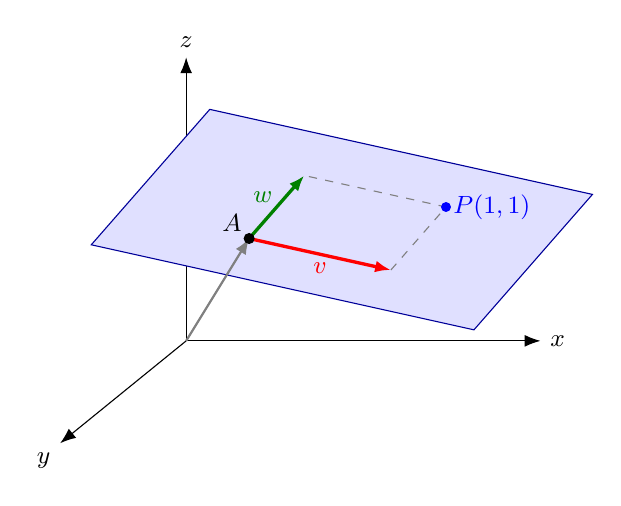
\begin{tikzpicture}[every node/.style={font=\small}, >={Latex[length=2mm]}]
	\draw[->] (0,0) -- (4.5,0) node[right] {$x$};
	\draw[->] (0,0) -- (0,3.6) node[above] {$z$};
	\draw[->] (0,0) -- (-1.6,-1.3) node[below left] {$y$};
	\fill[blue!12] (-1.205,1.22) -- (3.655,0.14) -- (5.16,1.86) -- (0.30,2.94) -- cycle;
	\draw[blue!60!black] (-1.205,1.22) -- (3.655,0.14) -- (5.16,1.86) -- (0.30,2.94) -- cycle;
	\draw[->, gray, thick] (0,0) -- (0.8,1.3);
	\draw[dashed, gray] (2.6,0.9) -- (3.3,1.7) -- (1.5,2.1);
	\draw[->, red, very thick] (0.8,1.3) -- (2.6,0.9) node[midway, below, inner sep=2.5pt] {$v$};
	\draw[->, green!50!black, very thick] (0.8,1.3) -- (1.5,2.1) node[midway, above left, inner sep=1pt] {$w$};
	\fill (0.8,1.3) circle (2pt) node[above left, inner sep=2.5pt] {$A$};
	\fill[blue] (3.3,1.7) circle (1.8pt) node[right, inner sep=2.5pt] {$P(1,1)$};
\end{tikzpicture}
\end{document}
